\vspace{-1pt}
\section{Introduction}
Community detection is a fundamental task in social network analysis~\cite{tang2010community}, which identifies sub-groups within social networks. These groups can represent a variety of things including karate club membership, political leanings, and deeply-held beliefs. Traditionally, these groups are identified by searching for densely-connected groups of nodes in the graph~\cite{malliaros2013clustering}. More recently, attributed approaches go beyond merely the links to cluster nodes based upon their attributes and their network connections~\cite{ruan2013efficient}. Existing community detection approaches suffer from a major flaw: the inability to assign lowly-connected users into communities. Despite the fact that lowly-connected users are not well-blended into the social network, the information they provide can be crucial for better understanding the motivations and beliefs of the community, especially considering there could be a long-tail of lowly-connected users. Failure to incorporate the lowly-connected users may result in biased results. For instance, studying groups within a social network, such as a Twitter retweet network, can be biased towards users whose tweets get a large number of retweets. This will lead to a biased analysis of the data in which not all users' voices are heard. Instead, those high-degree users with non-genuine retweets will end up having more voice in the study. Consider the toy example shown in Figure~\ref{pi}. Each node represents a user and the shapes represent difference of opinion in the network; the shade and different texture of each shape represent their variability of expressing opinions. Traditional community detection methods that solely focus on the highly-connected nodes would only capture the opinions of users within the dark-grey area; however, many diverse opinions are lost due to the fact that the users in the light grey area are excluded because of their low degree in the network.

The goal of this paper is twofold. First, we demonstrate empirically the existence of biases in existing community detection approaches using real-world datasets. Through the analysis, we show that current state-of-the-art community detection methods suffer from ignoring low-degree users that have few links either by failing to incorporate them, or by putting them into small groups which are then ignored in the study. These low-degree users have value to be included in the communities, as they offer a more diverse, nuanced representation of the communities. Second, to overcome this issue, we introduce a new community detection method, Communities with Lowly-connected Attributed Nodes (CLAN), that would mitigate the existence of this bias towards low-degree nodes.
\begin{figure}[H]
  \centering
  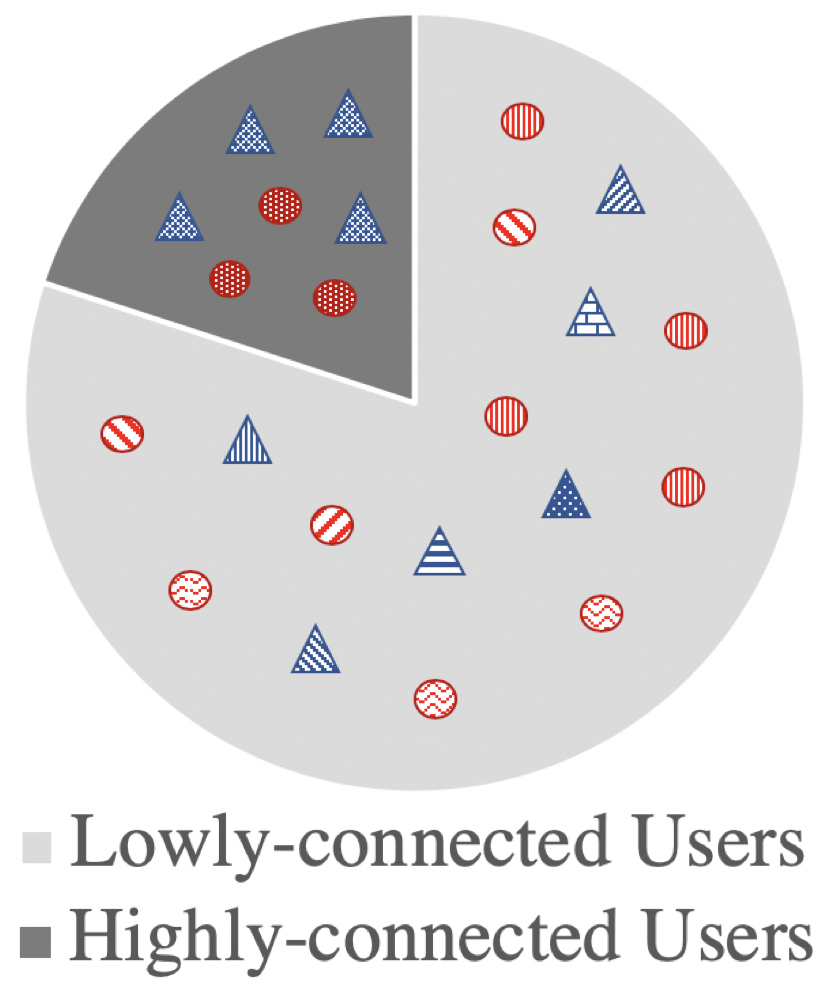
\includegraphics[width=0.28\textwidth]{pi7.png}
  \caption{Demonstration of versatility of relevant low-degree people in social networks who get ignored by biased community detection methods. Shapes (circle, triangle) represent opinion, and texture represents variations of the opinion. We provide real-world examples of how this manifests in subsequent sections.}
  \label{pi}
\end{figure}
%We prove our statement by conducting an experiment in which the state of the art methods are compared to a ground truth that was collected using human annotators and show the superiority of our method in terms of Jaccard similarity and F1 scores. To prove our point further, we use another dataset with a ground truth collected in a more automated fashion and demonstrate CLAN's ability in improving the results. 
Our contributions are as follows:
\begin{table*}
\begin{tabular}{ |p{1.5cm}||p{1.8cm}|p{5.3cm}||p{2cm}|p{4.7cm}|  }
 \hline
 \multicolumn{1}{|c||}{}&\multicolumn{2}{c||}{Gamergate Dataset}&\multicolumn{2}{c|}{U.S. Presidential Election Dataset}\\
 \hline
Method & Discarded Unique Hashtags &Examples& Discarded Unique Hashtags &Examples\\
 \hline
 CESNA   &597 (38.6\%)& \#gamerignorance,\#ethicsinjournalism, \#feministgate,\#sexismiswickedcool   & 1518 (66.9\%)&\#refugeeswelcome, \#Guns,\#OscarsStillSoWhite, \#TrumpDumped\\
 \hline
 Modularity&   625 (40.4\%) &\#misandricfeminists, \#violenceagainstwomen,\#gamersagainstgamergate, \#stopgamejournalism2014,  &302 (13.3\%)&\#Christians4Hillary,\#Killary, \#FakeHateCrimes, \#TrumpRiots \\
 \hline
\end{tabular}
\caption{Number of missed hashtags which can be representative of missing information along with some examples in biased methods.}
\label{hashtags}
\end{table*}
\begin{enumerate}
\item We introduce CLAN, a novel community detection approach that is able to categorize low-degree users into their relevant communities.
\item Through experimentation, we show that CLAN is able to outperform the existing state-of-the-art community detection methods in terms of predictive accuracy while still being able to classify more users. We conduct further experiments to test the resiliency of CLAN to different data regimes.
\item We demonstrate the existence of bias in community detection approaches that is introduced from ignoring low-degree users. We show that CLAN is able to overcome this challenge by classifying low-degree users. 

\end{enumerate}
\section{Biases in Community Detection Methods}
Analysis on community detection tends to focus on the largest communities. Methods that tend to exclude low-degree nodes are at greater risk of losing information in their detected significant communities. 
We demonstrate the existence of this bias by showing what is omitted by existing community detection approaches. We use two state-of-the-art approaches, CESNA~\cite{6729613}, and the Louvain method~\cite{blondel2008fast}. Louvain uses only the network while assigning communities, while CESNA uses both the network and user attributes. We apply these methods to two separate datasets, one based on Gamergate and one based on the 2016 U.S. Presidential Election. Both of these datasets contain two major contingents, and ground truth information (both datasets, and the methodology for obtaining ground truth, will be introduced in detail later). Table~\ref{hashtags} shows the information that is omitted by excluding the lowly-connected users. These statistics are taken by comparing the ground truth labels with the labels assigned by the community detection algorithm.
For example, in one of the methods, CESNA, %FM: which one?
the ``\#refugeeswelcome'' hashtag and the user who tweeted this hashtag remained unlabeled by the user being put in a small insignificant community from the election dataset, discussed in the later sections. By not including this user tweeting this hashtag, we lose this piece of information when we analyze the communities. In other words, degree is not correlated with relevancy to the topic and therefore merely degree and connections in social networks should not be indicative of community membership. Other examples of such are demonstrated in Table~\ref{hashtags}, such as the ``\#Christians4Hillary,'' ``\#gamersagainstgamergate,'' and many other hashtags of such type in two of the datasets that we will be using in this paper. The goal of this work is to introduce a method that would mitigate this bias by the inclusion of low-degree users into their correct belonging significant communities. 
